
\begin{figure}
  \def\frac{0.32}
    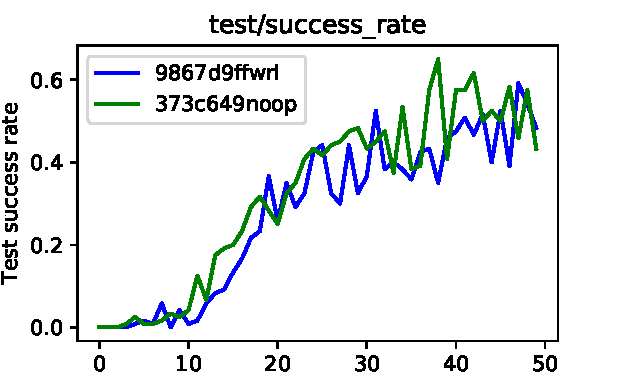
\includegraphics[width=\frac\columnwidth]{media/res/373c649_FetchSlide-v1-noop/test/success_rate.pdf}%
    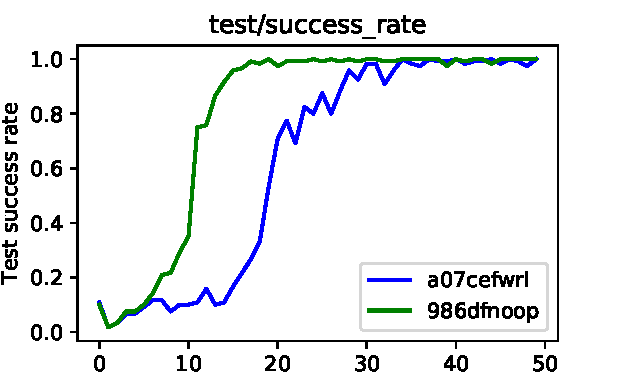
\includegraphics[width=\frac\columnwidth]{media/res/a077c9e_FetchPush-v1-fwrl/test/success_rate.pdf}%
    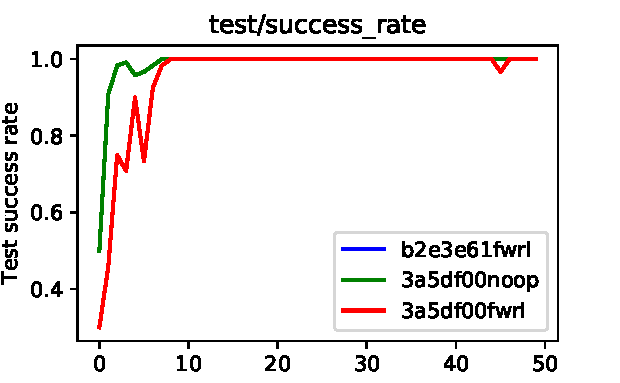
\includegraphics[width=\frac\columnwidth]{media/res/3a5df00_FetchReach-v1-fwrl/test/success_rate.pdf}\\
    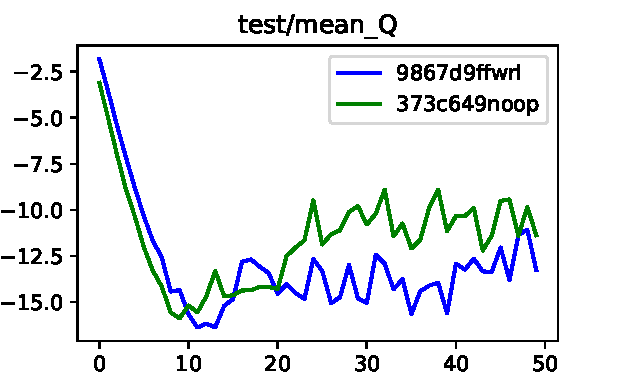
\includegraphics[width=\frac\columnwidth]{media/res/373c649_FetchSlide-v1-noop/test/mean_Q.pdf}%
    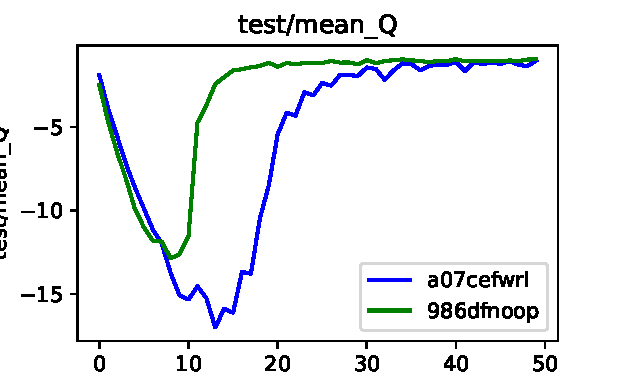
\includegraphics[width=\frac\columnwidth]{media/res/a077c9e_FetchPush-v1-fwrl/test/mean_Q.pdf}%
    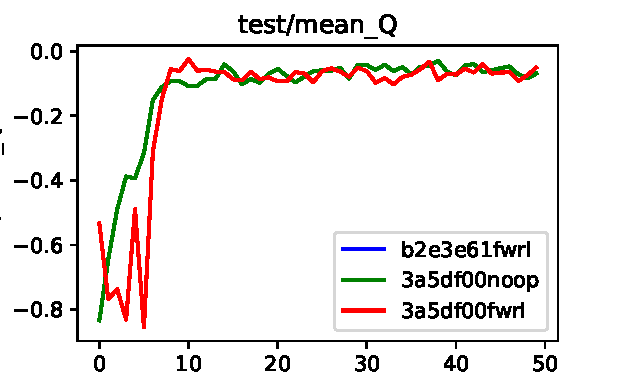
\includegraphics[width=\frac\columnwidth]{media/res/3a5df00_FetchReach-v1-fwrl/test/mean_Q.pdf}
    \caption{fwrl = Floyd Warshall ($=\Loss_{\text{ddpg}} +
      \Loss_{\text{upper}}$) with HER sampling;
      noop = DDPG ($=\Loss_{\text{ddpg}}$)with HER sampling.
  Test success rate and Mean Q on (1) Fetch-Slide, (2) Fetch-Push and (3)
  Fetch-Reach task. fwrl does consistently worse than HER.}
    \label{fig:fetch-slide-success}
\end{figure}


%
\begin{figure}%
  \def\frac{0.24}
  With HER sampling:\\
  \includegraphics[width=\frac\columnwidth]{media/res/3a90344-FetchReach-v1-stepfwrl-future/test/success_rate.pdf}%
  \includegraphics[width=\frac\columnwidth]{media/res/3a90344-FetchReach-v1-stepfwrl-future/test/mean_Q.pdf}%
  \includegraphics[width=\frac\columnwidth]{media/res/3a90344-FetchReach-v1-stepfwrl-future/train/critic_loss.pdf}%
  \includegraphics[width=\frac\columnwidth]{media/res/3a90344-FetchReach-v1-stepfwrl-future/train/critic_addnl_loss.pdf}\\
  Without HER sampling:\\
  \includegraphics[width=\frac\columnwidth]{media/res/d047a03-FetchReach-v1-stepfwrl-none/test/success_rate.pdf}%
  \includegraphics[width=\frac\columnwidth]{media/res/d047a03-FetchReach-v1-stepfwrl-none/test/mean_Q.pdf}%
  \includegraphics[width=\frac\columnwidth]{media/res/d047a03-FetchReach-v1-stepfwrl-none/train/critic_loss.pdf}%
  \includegraphics[width=\frac\columnwidth]{media/res/d047a03-FetchReach-v1-stepfwrl-none/train/critic_addnl_loss.pdf}\\
Using both upper and lower bound in FWRL\\
  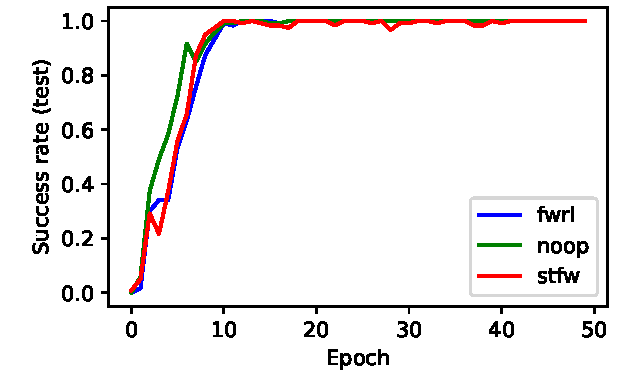
\includegraphics[width=\frac\columnwidth]{media/res/f0d4cfa-FetchReach-v1-stfw-none/test/success_rate.pdf}%
  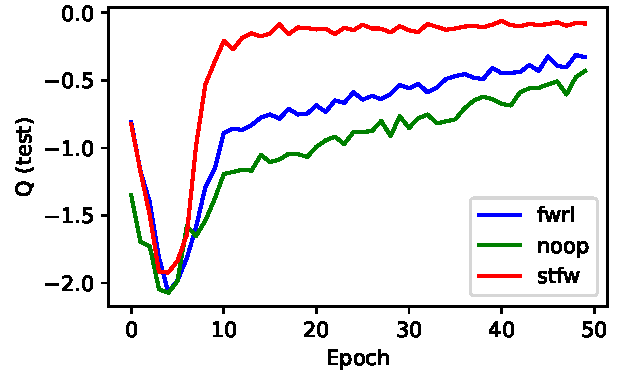
\includegraphics[width=\frac\columnwidth]{media/res/f0d4cfa-FetchReach-v1-stfw-none/test/mean_Q.pdf}%
  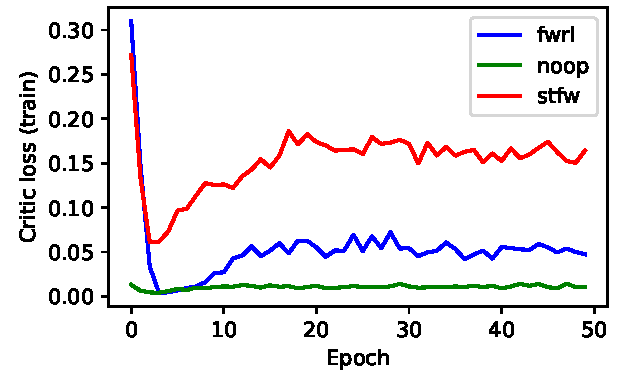
\includegraphics[width=\frac\columnwidth]{media/res/f0d4cfa-FetchReach-v1-stfw-none/train/critic_loss.pdf}%
  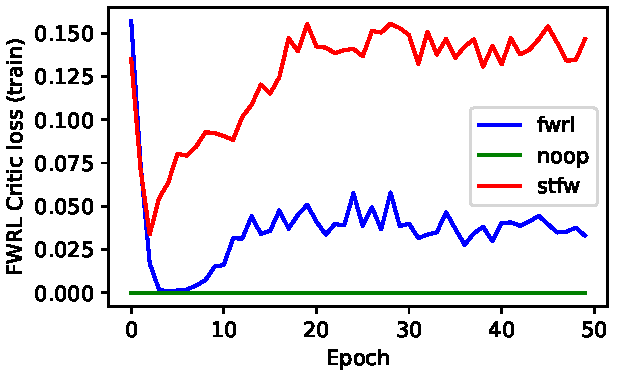
\includegraphics[width=\frac\columnwidth]{media/res/f0d4cfa-FetchReach-v1-stfw-none/train/critic_addnl_loss.pdf}\\
  \caption{
    stepfwrl = DDPG loss $\Loss_{\text{ddpg}}$ + Step loss $\Loss_{\text{step}}$
    + FWRL constraints $\Loss_{\text{upper}} + \Loss_{\text{lower}}$, noop =
    DDPG loss $\Loss_{\text{ddpg}}$  + HER
    sampling, fwrl = DDPG Loss $\Loss_{\text{ddpg}}$ + FWRL constraints $\Loss_{\text{upper}} + \Loss_{\text{lower}}$.
    All experiments on Fetch-Reach task.
  }%
  \label{fig:fwrl-stepfwrl-noop-FetchReach}%
\end{figure}%
% 

%
\begin{figure}%
  \def\frac{0.24}
  With HER sampling\\
  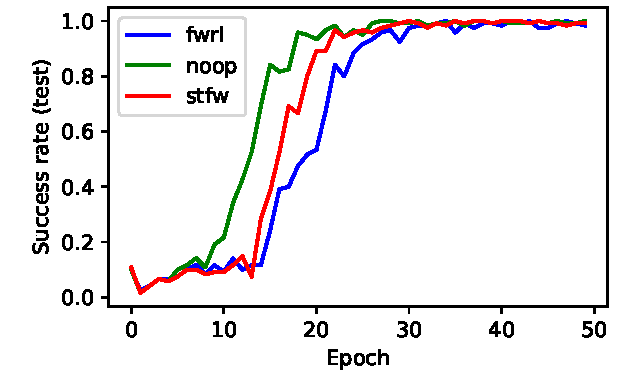
\includegraphics[width=\frac\columnwidth]{media/res/ea0e35b-FetchPush-v1-stfw-future/test/success_rate.pdf}%
  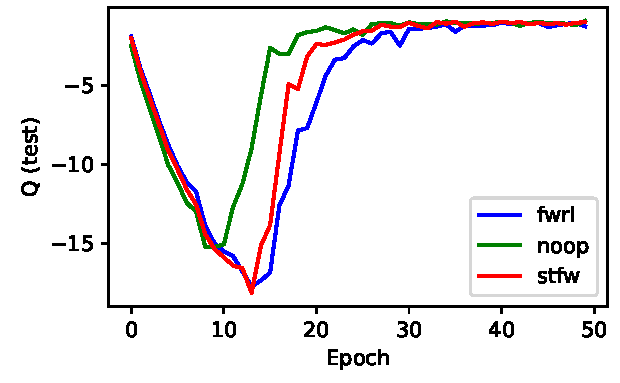
\includegraphics[width=\frac\columnwidth]{media/res/ea0e35b-FetchPush-v1-stfw-future/test/mean_Q.pdf}%
  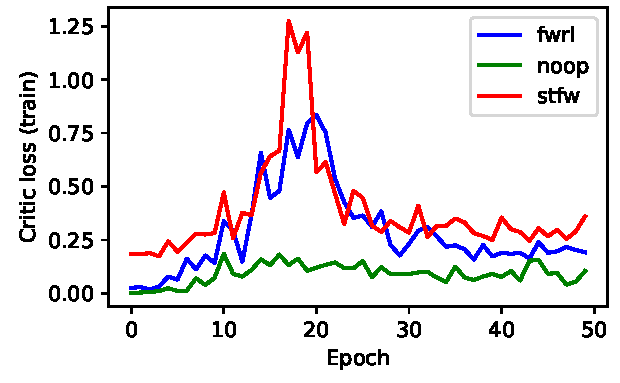
\includegraphics[width=\frac\columnwidth]{media/res/ea0e35b-FetchPush-v1-stfw-future/train/critic_loss.pdf}%
  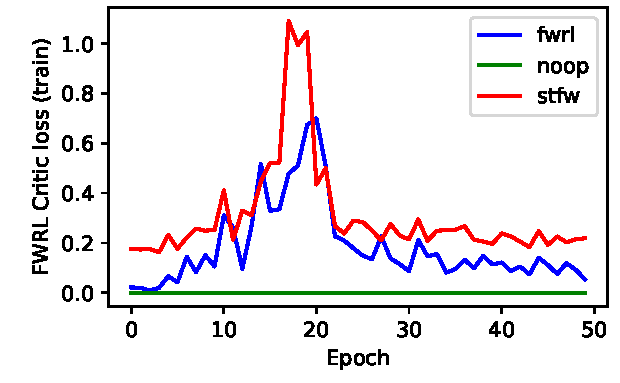
\includegraphics[width=\frac\columnwidth]{media/res/ea0e35b-FetchPush-v1-stfw-future/train/critic_addnl_loss.pdf}\\
  Without HER sampling\\
  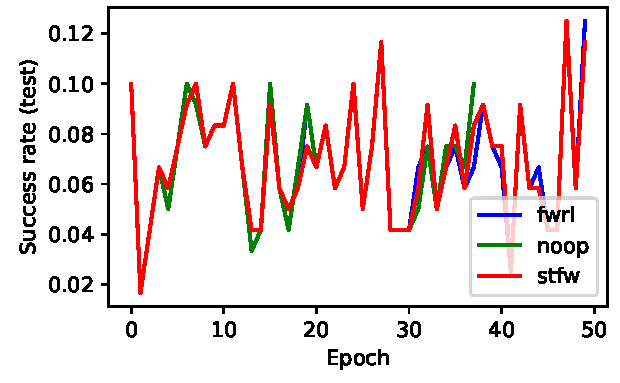
\includegraphics[width=\frac\columnwidth]{media/res/ea0e35b-FetchPush-v1-stfw-none/test/success_rate.pdf}%
  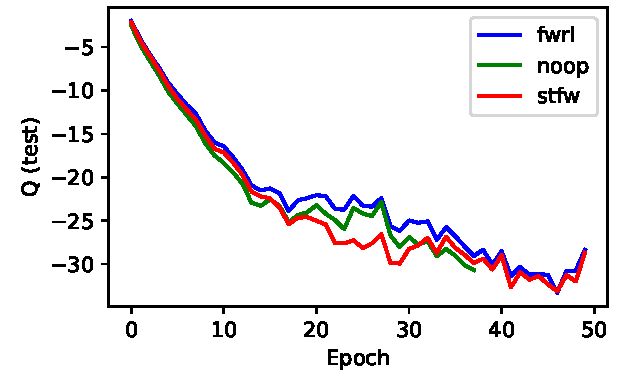
\includegraphics[width=\frac\columnwidth]{media/res/ea0e35b-FetchPush-v1-stfw-none/test/mean_Q.pdf}%
  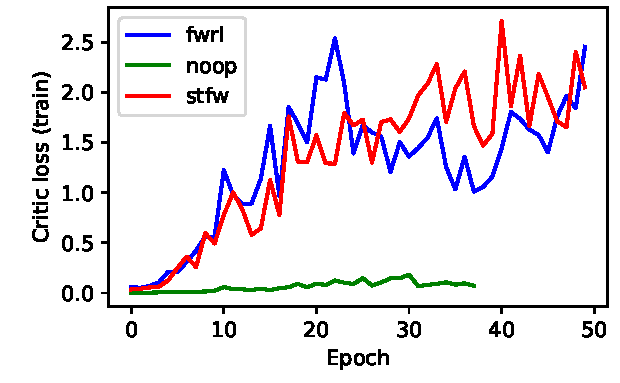
\includegraphics[width=\frac\columnwidth]{media/res/ea0e35b-FetchPush-v1-stfw-none/train/critic_loss.pdf}%
  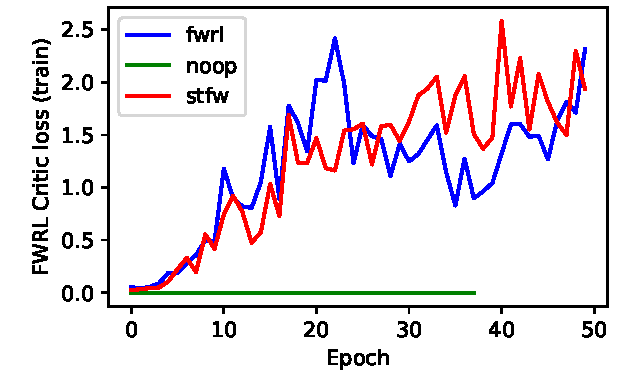
\includegraphics[width=\frac\columnwidth]{media/res/ea0e35b-FetchPush-v1-stfw-none/train/critic_addnl_loss.pdf}%
  \caption{stepfwrl = DDPG loss $\Loss_{\text{ddpg}}$ + Step loss $\Loss_{\text{step}}$
    + FWRL constraints $\Loss_{\text{upper}} + \Loss_{\text{lower}}$, noop =
    DDPG loss $\Loss_{\text{ddpg}}$  + HER
    sampling, fwrl = DDPG Loss $\Loss_{\text{ddpg}}$ + FWRL constraints $\Loss_{\text{upper}} + \Loss_{\text{lower}}$.
    All experiments on Fetch-Push}
  \label{fig:loss-func-fetch-push}
\end{figure}
%

%
\begin{figure}
  \def\frac{0.32}
Loss function breakdown without HER sampling on Fetch Push\\
  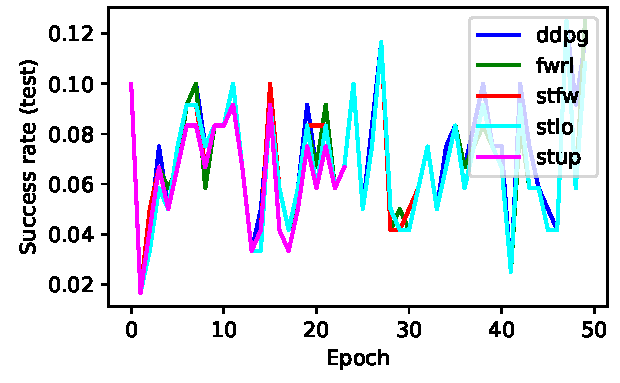
\includegraphics[width=\frac\columnwidth]{media/res/f84daa7-FetchPush-v1-stfw-none/test/success_rate.pdf}%
  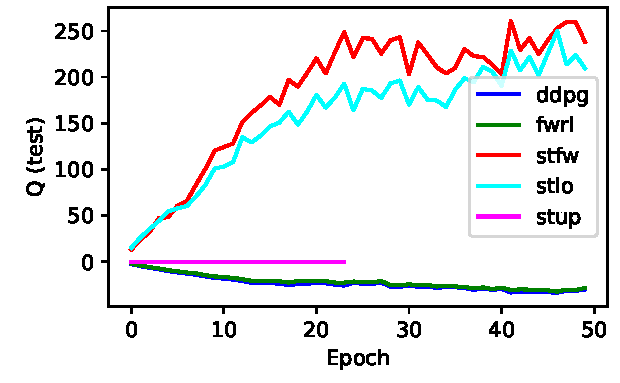
\includegraphics[width=\frac\columnwidth]{media/res/f84daa7-FetchPush-v1-stfw-none/test/mean_Q.pdf}%
  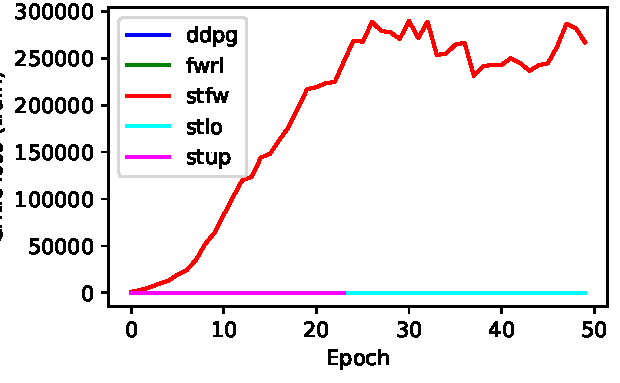
\includegraphics[width=\frac\columnwidth]{media/res/f84daa7-FetchPush-v1-stfw-none/train/critic_loss.pdf}\\
Loss function breakdown with HER sampling on Fetch Push\\
  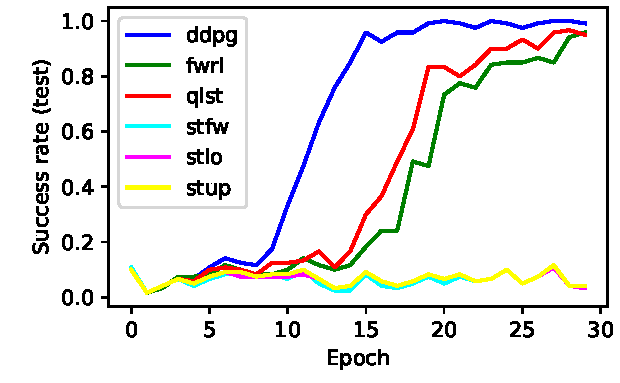
\includegraphics[width=\frac\columnwidth]{media/res/3f1eafe-FetchPush-v1-stfw-future/test/success_rate.pdf}%
  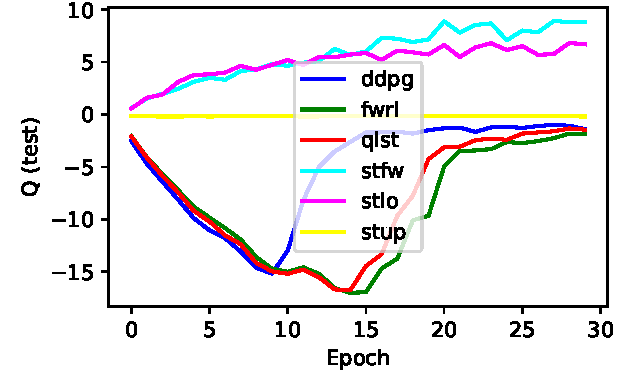
\includegraphics[width=\frac\columnwidth]{media/res/3f1eafe-FetchPush-v1-stfw-future/test/mean_Q.pdf}%
  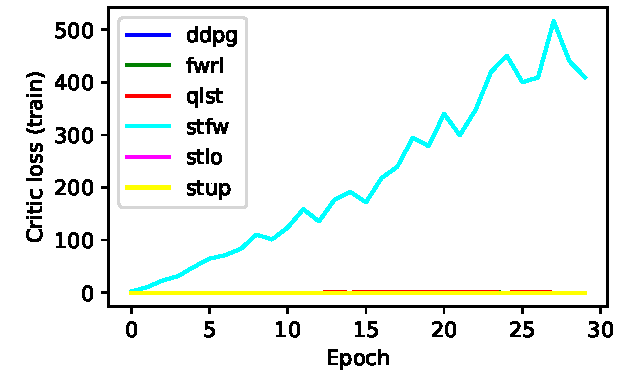
\includegraphics[width=\frac\columnwidth]{media/res/3f1eafe-FetchPush-v1-stfw-future/train/critic_loss.pdf}%
  \caption{
    Fetch Push results. Loss function changes do no seem to make a difference.
    There are four parts to the loss function (1) DDPG Loss $\Loss_{\text{ddpg}}$ ,
    (2) Step loss$\Loss_{\text{step}}$,  
    (3) Lower bound $\Loss_{\text{lower}}$ and
    (4) Upper bound $\Loss_{\text{upper}}$ .
    ddpg = $\Loss_{\text{ddpg}}$,
    dqst = $\Loss_{\text{ddpg}}$ + $\Loss_{\text{step}}$,
    fwrl = $\Loss_{\text{ddpg}}$ + $\Loss_{\text{lower}}$ +
    $\Loss_{\text{upper}}$,
    qlst = $\Loss_{\text{ddpg}}$ + $\Loss_{\text{step}}$ + $\Loss_{\text{lower}}$ + $\Loss_{\text{upper}}$.
    stfw = $\Loss_{\text{step}}$ + $\Loss_{\text{lower}}$ + $\Loss_{\text{upper}}$,
    stlo = $\Loss_{\text{step}}$ + $\Loss_{\text{lower}}$,
    stup = $\Loss_{\text{step}}$ + $\Loss_{\text{upper}}$.
    Success rate is the fraction of times the agent reaches the goal. Q(test) is
    the estimated cumulative reward by the network. Critic loss is the total
    loss plotted during training.
    Because stfw, stlo, stup fail to succeed, we infer that the $\Loss_{\text{ddpg}}$ DDPG loss is
    critical for making the algorithm work. Since the qlst works better than
    fwrl, we infer that $\Loss_{\text{step}}$ Step loss is also important.
    only.
    Since there is slight improvement in dqst over ddpg, this means
    $\Loss_{\text{step}}$ really helps. dqst did not run fully but it shows
    promise (I need to fix a bug).
    But why does the loss for stfw keep rising? Does it mean that the SGD is not
    able to optimize the loss gradients in the right direction?
  }%
  \label{fig:fwrl-stepfwrl-noop-FetchPush}%
\end{figure}%
% 